\begin{center}

\includegraphics[width=0.6\textwidth]{content/3/chapter4/images/41.png}\\
Cippi slides down the slide
\end{center}

With C++20, lambda expressions support template parameters and hence concepts, can be defaultconstructed and support copy assignment when they have no state. Additionally, lambda expressions can be used in unevaluated contexts. With C++20, they detect when you implicitly copy the this pointer. This means a significant cause of undefined behavior with lambdas is gone.

Let’s start with template parameters for lambdas.


\subsubsubsection{4.7.1\hspace{0.2cm} Template Parameter for Lambdas}

Admittedly, the differences between typed lambdas (C++11), generic lambdas (C++14), and template lambdas (template parameter for lambdas) in C++20 are subtle.

\noindent
Typed lambdas, generic lambdas, and template lambdas
\begin{lstlisting}[style=styleCXX]
// templateLambda.cpp

#include <iostream>
#include <string>
#include <vector>

auto sumInt = [](int fir, int sec) { return fir + sec; };
auto sumGen = [](auto fir, auto sec) { return fir + sec; };
auto sumDec = [](auto fir, decltype(fir) sec) { return fir + sec; };
auto sumTem = []<typename T>(T fir, T sec) { return fir + sec; };

 int main() {
	
	 std::cout << '\n';
	
	 std::cout << "sumInt(2000, 11): " << sumInt(2000, 11) << '\n';
	 std::cout << "sumGen(2000, 11): " << sumGen(2000, 11) << '\n';
	 std::cout << "sumDec(2000, 11): " << sumDec(2000, 11) << '\n';
	 std::cout << "sumTem(2000, 11): " << sumTem(2000, 11) << '\n';
	
	 std::cout << '\n';
	
	 std::string hello = "Hello ";
	 std::string world = "world";
	 // std::cout << "sumInt(hello, world): " << sumInt(hello, world) << '\n';
	 std::cout << "sumGen(hello, world): " << sumGen(hello, world) << '\n';
	 std::cout << "sumDec(hello, world): " << sumDec(hello, world) << '\n';
	 std::cout << "sumTem(hello, world): " << sumTem(hello, world) << '\n';
	
	
	 std::cout << '\n';
	
	 std::cout << "sumInt(true, 2010): " << sumInt(true, 2010) << '\n';
	 std::cout << "sumGen(true, 2010): " << sumGen(true, 2010) << '\n';
	 std::cout << "sumDec(true, 2010): " << sumDec(true, 2010) << '\n';
	 // std::cout << "sumTem(true, 2010): " << sumTem(true, 2010) << '\n';
	
	 std::cout << '\n';
	
}
\end{lstlisting}

Before I show the presumably astonishing output of the program, I want to compare the four lambdas.

\begin{itemize}
\item 
sumInt
\begin{itemize}
\item 
C++11

\item 
Typed lambda

\item 
Accepts only types convertible to int
\end{itemize}

\item 
sumGen
\begin{itemize}
\item 
C++14

\item 
Generic lambda

\item 
Accepts all types
\end{itemize}

\item 
sumDec
\begin{itemize}
\item 
C++14

\item 
Generic lambda

\item 
The second type must be convertible to the first type
\end{itemize}

\item 
sumTem
\begin{itemize}
\item 
C++20

\item 
Template lambda

\item 
The first type and the second type must be identical
\end{itemize}
\end{itemize}

What does this mean for template arguments with different types? Of course, each lambda accepts int (lines 16 - 19), and the typed lambda sumInt does not accept strings (line 25).

Invoking the lambdas with the bool true and the int 2010 may be surprising (lines 33 - 36).

\begin{itemize}
\item 
sumInt returns 2011 because true is an integral, promoted to int.

\item 
sumGen returns 2011 because true is an integral, promoted to int. There is a subtle difference between sumInt and sumGen, which I will present in a few lines.

\item 
sumDec returns 2. Why? The type of the second parameter sec becomes the type of the first parameter fir: thanks to decltype(fir) sec, the compiler deduces the type of fir and makes it the type of sec. Consequently, 2010 is converted to true. In the expression fir + sec, fir is integral promoted to 1. Finally, the result is 2.

\item 
sumTem is not valid.
\end{itemize}

\begin{tcblisting}{commandshell={}}
sumInt(2000, 11): 2011
sumGen(2000, 11): 2011
sumDec(2000, 11): 2011
sumTem(2000, 11): 2011

sumGen(hello, world): Hello world
sumDec(hello, world): Hello world
sumTem(hello, world): Hello world

sumInt(true, 2010): 2011
sumGen(true, 2010): 2011
sumDec(true, 2010): 2
\end{tcblisting}

\begin{center}
The subtle differences between typed lambdas, generic lambdas, and template lambdas
\end{center}

A more typical use case for template lambdas is the use of containers in lambdas. The following program presents three lambdas accepting a container. Each lambda returns the size of the container.

\noindent
Three lambdas accepting a container
\begin{lstlisting}[style=styleCXX]
// templateLambdaVector.cpp

#include <concepts>
#include <deque>
#include <iostream>
#include <string>
#include <vector>

auto lambdaGeneric = [](const auto& container) { return container.size(); };
auto lambdaVector = []<typename T>(const std::vector<T>& vec) { return vec.size(); };
auto lambdaVectorIntegral = []<std::integral T>(const std::vector<T>& vec) {
	return vec.size();
};

 int main() {
	
	
	std::cout << '\n';
	
	std::deque deq{1, 2, 3};
	std::vector vecDouble{1.1, 2.2, 3.3, 4.4};
	std::vector vecInt{1, 2, 3, 4, 5};
	
	std::cout << "lambdaGeneric(deq): " << lambdaGeneric(deq) << '\n';
	// std::cout << "lambdaVector(deq): " << lambdaVector(deq) << '\n';
	// std::cout << "lambdaVectorIntegral(deq): "
	// << lambdaVectorIntegral(deq) << '\n';
	
	std::cout << '\n';
	
	std::cout << "lambdaGeneric(vecDouble): " << lambdaGeneric(vecDouble) << '\n';
	std::cout << "lambdaVector(vecDouble): " << lambdaVector(vecDouble) << '\n';
	// std::cout << "lambdaVectorIntegral(vecDouble): "
	// << lambdaVectorIntegral(vecDouble) << '\n';
	
	std::cout << '\n';
	
	std::cout << "lambdaGeneric(vecInt): " << lambdaGeneric(vecInt) << '\n';
	std::cout << "lambdaVector(vecInt): " << lambdaVector(vecInt) << '\n';
	std::cout << "lambdaVectorIntegral(vecInt): "
	<< lambdaVectorIntegral(vecInt) << '\n';
	
	std::cout << '\n';
	
	}
\end{lstlisting}

Function lambdaGeneric (line 9) can be invoked with any data type that has a member function size(). Function lambdaVector (line 10) is more specific: it only accepts a std::vector. Function lambdaVectorIntegral (line 11) uses the C++20 concept std::integral. Consequently, it only accepts a std::vector using integral types such as int. To use the concept std::integral, I have to include the header <concepts>. I assume the small program is self-explanatory.

\begin{tcblisting}{commandshell={}}
lambdaGeneric(deq): 3

lambdaGeneric(vecDouble): 4
lambdaVector(vecDouble): 4

lambdaGeneric(vecInt): 5
lambdaVector(vecInt): 5
lambdaVectorIntegral(vecInt): 5
\end{tcblisting}

\begin{center}
Lambdas, accepting a container and a std::vector
\end{center}

\begin{tcolorbox}[colback=mygreen!5!white,colframe=mygreen!75!black,title={Class Template Argument Deduction}]
There is one feature in the program templateLambdaVector.cpp that you have probably missed. Since C++17, the compiler can deduce the type of a class template from its arguments (lines 20 - 22). Consequently, instead of the verbose std::vector<int> myVec{1, 2, 3} you can simply write std::vector myVec{1, 2, 3}.
\end{tcolorbox}

\subsubsubsection{4.7.2\hspace{0.2cm} Detection of the Implicit Copy of the this Pointer}

The C++20 compiler detects when you implicitly copy the this pointer. Implicitly capturing the this pointer by copy can cause undefined behavior. Undefined behavior essentially means that there are no guarantees for the behavior of the program, such as for the following:

\noindent
Implicitly capturing the this pointer by copy
\begin{lstlisting}[style=styleCXX]
// lambdaCaptureThis.cpp

#include <iostream>
#include <string>

struct LambdaFactory {
	auto foo() const {
		return [=] { std::cout << s << '\n'; };
	}
	std::string s = "LambdaFactory";
	~LambdaFactory() {
		std::cout << "Goodbye" << '\n';
	}
};

auto makeLambda() {
	LambdaFactory lambdaFactory; \
	
	return lambdaFactory.foo();
}


int main() {

	std::cout << '\n';
	
	auto lam = makeLambda();
	lam();
	
	std::cout << '\n';

}
\end{lstlisting}

The compilation of the program works as expected, but this does not hold for the execution of the program.

\begin{center}
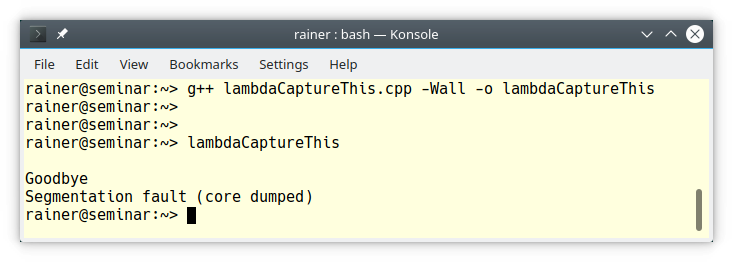
\includegraphics[width=0.6\textwidth]{content/3/chapter4/images/42.png}\\
Segmentation fault due to undefined behavior
\end{center}

Do you spot the issue in the program lambdaCaptureThis.cpp? The member function foo (line 7) returns the lambda [=] { std::cout << s << '\verb|\|n'; } having an implicit copy of the this pointer. This implicit copy is no issue in (line 17), but it becomes an issue with the end of the scope. The end of the scope means the end of the lifetime of the local lambda (line 19). Consequently, the call lam() (line 28) triggers undefined behavior.

A C++20 compiler must, in this case, issue a warning.

\begin{center}
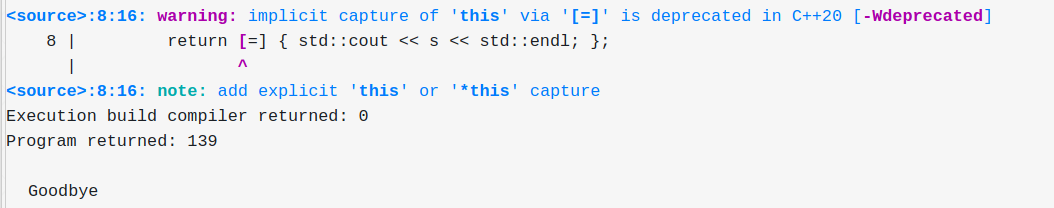
\includegraphics[width=0.6\textwidth]{content/3/chapter4/images/1-8.png}\\
C++20 diagnoses a warning
\end{center}

The last two lambdas features of C++20 are quite handy when you combine them: Lambdas in C++20 can be default-constructed and support copy-assignment when they have no state. Additionally, lambdas can be used in unevaluated contexts.

\subsubsubsection{4.7.3\hspace{0.2cm} Lambdas in an Unevaluated Context and Stateless Lambdas can be Default-Constructed and Copy-Assigned}

Admittedly, the title of this section contains two terms that may be new to you: unevaluated context and stateless lambda. Let me start with unevaluated context.

\noindent
4.7.3.1\hspace{0.2cm} Unevaluated Context

The following code snippet has a function declaration and a function definition.

\noindent
Declaration and definition of a function
\begin{lstlisting}[style=styleCXX]
int add1(int, int); // declaration
int add2(int a, int b) { return a + b; } // definition
\end{lstlisting}

Function add1 is declared, while add2 is defined. This means, if you use add1 in an evaluated context, for example, by invoking it, you get a link-time error. The key observation is that you can use add1 in unevaluated contexts, such as \href{https://en.cppreference.com/w/cpp/language/typeid}{typeid} or \href{https://en.cppreference.com/w/cpp/language/decltype}{decltype}. Both operators accept unevaluated operands.

\noindent
Unevaluated context
\begin{lstlisting}[style=styleCXX]
// unevaluatedContext.cpp

#include <iostream>
#include <typeinfo> // typeid

int add1(int, int); // declaration
int add2(int a, int b) { return a + b; } // definition

int main() {
	
	std::cout << '\n';
	
	std::cout << "typeid(add1).name(): " << typeid(add1).name() << '\n';
	
	decltype(*add1) add = add2;
	
	std::cout << "add(2000, 20): " << add(2000, 20) << '\n';
	
	std::cout << '\n';

}
\end{lstlisting}

typeid(add1).name() (line 13) returns a string representation of the type and decltype (line 15) deduces the type of its argument.


\begin{center}
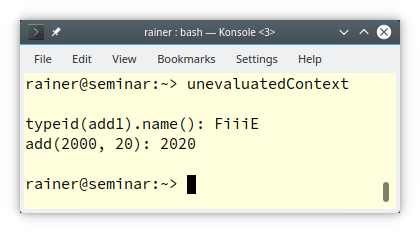
\includegraphics[width=0.6\textwidth]{content/3/chapter4/images/43.png}\\
Use of an unevaluated context
\end{center}

\noindent
4.7.3.2\hspace{0.2cm} Stateless Lambda

A stateless lambda is a lambda that captures nothing from its environment. Or, to put it another way, a stateless lambda is a lambda where the initial brackets [] in the lambda definition are empty. For example, the lambda expression auto add = [ ](int a, int b) { return a + b; }; is stateless.

\noindent
4.7.3.3\hspace{0.2cm} Adapting Associative Containers of the Standard Template Library

Before I show you the example, I have to add a few remarks. Container std::set and all other ordered associative containers from the Standard Template Library (std::map, std::multiset, and std::multimap) by default use the function object std::less to sort the keys. std::less sorts all keys lexicographically in ascending order. The declaration of \href{https://en.cppreference.com/w/cpp/container/set}{std::set} shows the implicit usage of std::less

\noindent
Declaration of std::set
\begin{lstlisting}[style=styleCXX]
template<
	class Key,
	class Compare = std::less<Key>,
	class Allocator = std::allocator<Key>
> class set;
\end{lstlisting}

Now, let me play with the ordering.

\noindent
Lambdas used in an unevaluated context
\begin{lstlisting}[style=styleCXX]
// lambdaUnevaluatedContext.cpp

#include <cmath>
#include <iostream>
#include <memory>
#include <set>
#include <string>

template <typename Cont>
void printContainer(const Cont& cont) {
	for (const auto& c: cont) std::cout << c << " ";
	std::cout << "\n";
}

 int main() {
	
	std::cout << '\n';
	
	std::set<std::string> set1 = {"scott", "Bjarne", "Herb", "Dave", "michael"};
	printContainer(set1);
	
	using SetDecreasing = std::set<std::string,
									decltype([](const auto& l, const auto& r) {
	 									return l > r;
									})>;
	SetDecreasing set2 = {"scott", "Bjarne", "Herb", "Dave", "michael"};
	printContainer(set2);
	
	using SetLength = std::set<std::string,
							decltype([](const auto& l, const auto& r) {
	 							return l.size() < r.size();
							})>;
	SetLength set3 = {"scott", "Bjarne", "Herb", "Dave", "michael"};
	printContainer(set3);
	
	std::cout << '\n';
	
	std::set<int> set4 = {-10, 5, 3, 100, 0, -25};
	printContainer(set4);
	
	using setAbsolute = std::set<int, decltype([](const auto& l, const auto& r) {
	 												return std::abs(l)< std::abs(r);
	})>;
	setAbsolute set5 = {-10, 5, 3, 100, 0, -25};
	printContainer(set5);
	
	std::cout << "\n\n";

}
\end{lstlisting}

set1 (line 19) and set4 (line 38) sort their keys in ascending order. Each of set2 (line 26), set3 (line 33), and set5 (line 44) sorts its keys in an unique manner, using a lambda in an unevaluated context. The using keyword (line 22) declares a type alias, which is used in the following line (line 26) to define the sets. Creating the std::set causes the call of the default constructor of the stateless lambda.

Here is the output of the program.

\begin{tcblisting}{commandshell={}}
Bjarne Dave Herb michael scott
scott michael Herb Dave Bjarne
Herb scott Bjarne michael

-25 -10 0 3 5 100
0 3 5 -10 -25 100
\end{tcblisting}

\begin{center}
Use of a lambda in an unevaluated context
\end{center}

When you study the output of the program, you may be surprised. The special set3, which uses the lambda [](const auto\& l, const auto\& r){ return l.size() < r.size(); } as a predicate, ignores the name Dave. The reason is simple. Dave has the same size as Herb, that was added first. std::set supports unique keys, and the keys are in this case identical using the special predicate. If I had used std::multiset, this wouldn’t have happened.

\begin{tcolorbox}[colback=mygreen!5!white,colframe=mygreen!75!black,title={Distilled Information}]
With C++20, lambdas can have template parameters. In addition, lambdas detect when the this pointer is implicitly referenced.
\end{tcolorbox}










